In this section the system described will be modelled and validated using the AlloyTools framework, the analysis is divided in 4 main parts
\begin{itemize}
    \item Static Analysis
    \item Dynamic Analysis
    \item Assertions
    \item Word Generation
\end{itemize}
For this analysis the following assumption has been considered
\begin{itemize}
    \item The Float type (not defined) represent a decimal number
    \item A CPO can be modelled without being a part of the EMSP
\end{itemize}

\subsection{Static Analysis}
Here the model is created, all the classes are represented by a sig, for the purpose of this analysis only the relational property are considered, so the attribute of a basic type (such as Int,float,boolean,Data etc. etc.) are not considered.
This decision has been taken to simplify the model view and coding, most system that could be used to implement this system already support this type of data, or can be easily implemented and limited in their value ranges.//
As a guideline the type are written only in the declarations in a comment, they are defined by abstract type (not implemented) and their ranges are specified; this types are not considered in the rest of the document.

\begin{verbatim}
module eMall

//-------SIG-----

sig CPO{
cpms: set CPMS}

sig EMSP{
	users: set User,
	charges: set Charge,
	cpos:set CPO
}

sig CPMS{
	stations:set ChargingStation,
	maintainers:set Maintainer
}

abstract sig Person{
	//name: one Str,
	//surname: one Str,
 	//birthday: one Date,
    //mail: one Str,
 	//password: one Str,
} 
sig User extends Person{
	vehicles: set Vehicle
}
sig Maintainer extends Person{}

sig Vehicle{
	//batteryLevel: one Float,
	//KWperKm: one Float,
	location: one Location,
}{ 
//inRange[batteryLevel, 0, 100]
//inRange[KWperKm, 0, 100]
}

sig ChargingStation{
	position:one Location,
	//batteryPresent: one Bool,
	//batteryKWh: one Float,
	sockets: set ChargingSocket,
	strategy: one Strategy
} 
{  
    //batteryPresent.isTrue implies inRange[batteryKWh, 0, 100]
}

sig ChargingSocket{
	chargingType: one ChargingType,
	//available: one Bool,
	//maximumPowerAmount: one Float,
	energySource:one EnergySource
}{ 
    //inRange[maximumPowerAmount, 0, 100]
}

sig Charge{
	//paid: one Bool,
	station: one ChargingStation,
	user: one User
	//amount: one Float,
	//date: one Date
}{
    //amount>0
}

abstract sig Strategy{}
one sig Manual extends Strategy{}
one sig Automatic extends Strategy{}

abstract sig ChargingType{}
one sig SuperFast extends ChargingType{}
one sig Fast extends ChargingType{}
one sig Normal extends ChargingType{}

abstract sig EnergySource{}
sig Battery extends EnergySource{
//capacity: one Float
}{
    //capacity>0
}
sig DSO extends EnergySource{}


//utils types

//sig Date{}

//sig Str{}

//simplified using int
sig Location{  
//	latitude: one Int,   
//	longitude: one Int
}{//  inRange[latitude, -90, 90] and   
//	inRange[longitude, -180, 180]
}

//-------FACTS------

//fact uniqueMailForUser{
//	no disjoint u1,u2: User | u1.mail = u2.mail}

fact uniqueLocationForStation{
	no disjoint s1,s2: ChargingStation | s1.position = s2.position}

fact uniqueCPOForCPMS{
	no disjoint c1,c2: CPO, cp:CPMS | cp in c1.cpms and cp in c2.cpms}

fact uniqueStationForCPMS{
	no disjoint c1,c2: CPMS, s:ChargingStation | s in c1.stations and s in c2.stations}

fact socketOnlyOneStation{
all s:ChargingSocket| s in ChargingStation.sockets
no disjoint c1,c2: ChargingStation, 
s:ChargingSocket|(s in c1.sockets and s in c2.sockets)}

fact noVehicleWithoutUser{
	all v:Vehicle|  v in User.vehicles}

fact noStationWithoutCPMS{
	all s:ChargingStation|  s in CPMS.stations}

fact noUserWithoutEMSP{
	all u:User|  u in EMSP.users}

fact noChargeWithoutEMSP{
	all c:Charge|  c in EMSP.charges}

fact noChargeWithoutUserInTheEMSP{
	all c:Charge| c in EMSP.charges and c.user in EMSP.users
}

fact allChargeAreFromChargingStationInTheSystem{
	all s:Charge.station | s in EMSP.cpos.cpms.stations 
}
fact maintainersMantainStationOfTheSameCPO{
all m:Maintainer, c1,c2:CPO|(not c1=c2 and m in c1.cpms.maintainers) 
implies m not in c2.cpms.maintainers 
}
\end{verbatim}

\subsection{Dynamic Programming}
In this part the major operation are described and run, as a convection letter1 represent the old version (before the execution), while letter0 is the new version after the execution of the predicate.

\subsubsection{User books a charge}
\begin{verbatim}
    pred UserCreatesACharge(e,e1:EMSP,u:User, s:ChargingStation){
        one c:Charge  | u in e1.users and
        c.user=u and c.station=s and  (not (e1 = e)) and  e1.users=e.users and
        e1.cpos=e.cpos and e1.charges=e.charges+c
        }
        run UserCreatesACharge for 3 but exactly 2 EMSP    
\end{verbatim}

\begin{figure}[H]
    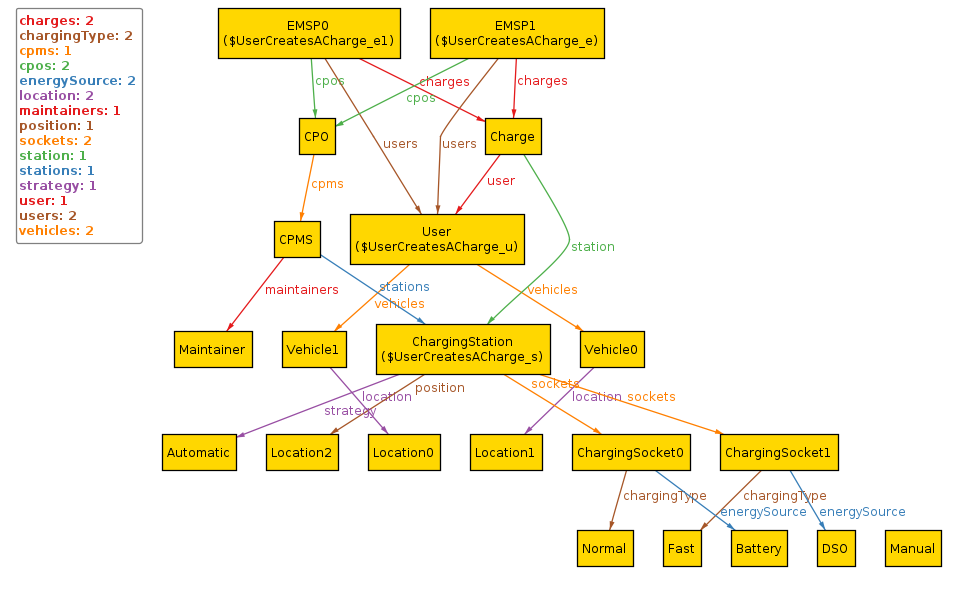
\includegraphics[keepaspectratio, width=16cm]{Alloy/UserCreatesCharge.png}
    \caption{Added Charge}
\end{figure}

\subsubsection{CPO subscribe to EMSP}
\begin{verbatim}
    pred CPOSubscribeItselfToEMSP(e,e1:EMSP,cpo:CPO){
        not (e1 = e)
       e.charges=e1.charges
       e.users= e1.users
       e.cpos=e1.cpos+cpo
       }
       run CPOSubscribeItselfToEMSP for 3 but exactly 2 EMSP, exactly 2 CPO           
\end{verbatim}
\begin{figure}[H]
    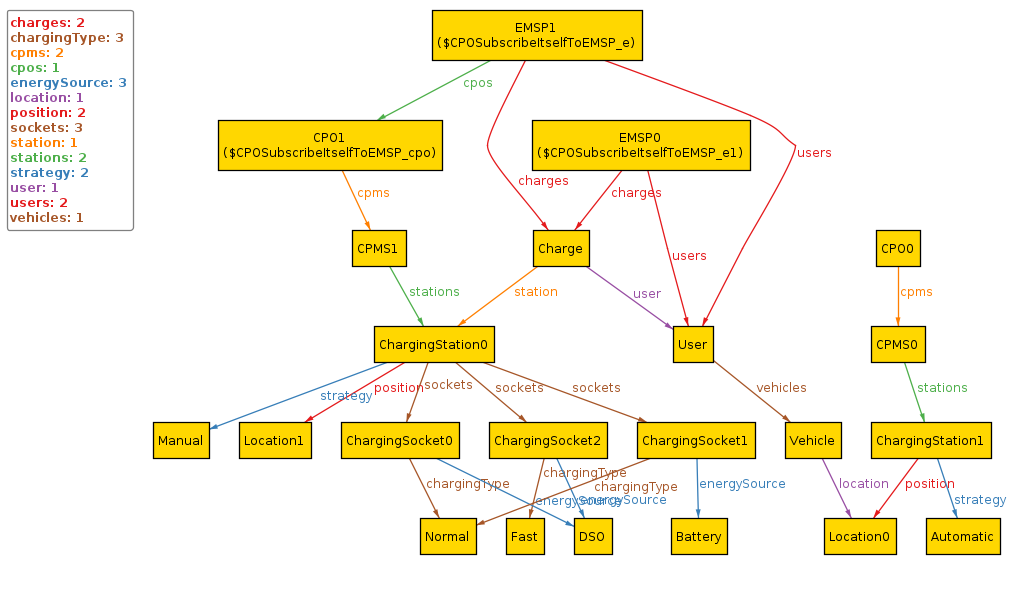
\includegraphics[keepaspectratio, width=16cm]{Alloy/CpoSubscribetoEMSP.png}
    \caption{CPO subscribed}
\end{figure}

\subsubsection{CPO add CPMS}
\begin{verbatim}
    pred CPOAddCPMS(c,c1:CPO,cp:CPMS){
        not (c1 = c)
       c.cpms=c1.cpms+cp
       }
       run CPOAddCPMS for 3 but exactly 2 CPO, exactly 2 CPMS    
\end{verbatim}
\begin{figure}[H]
    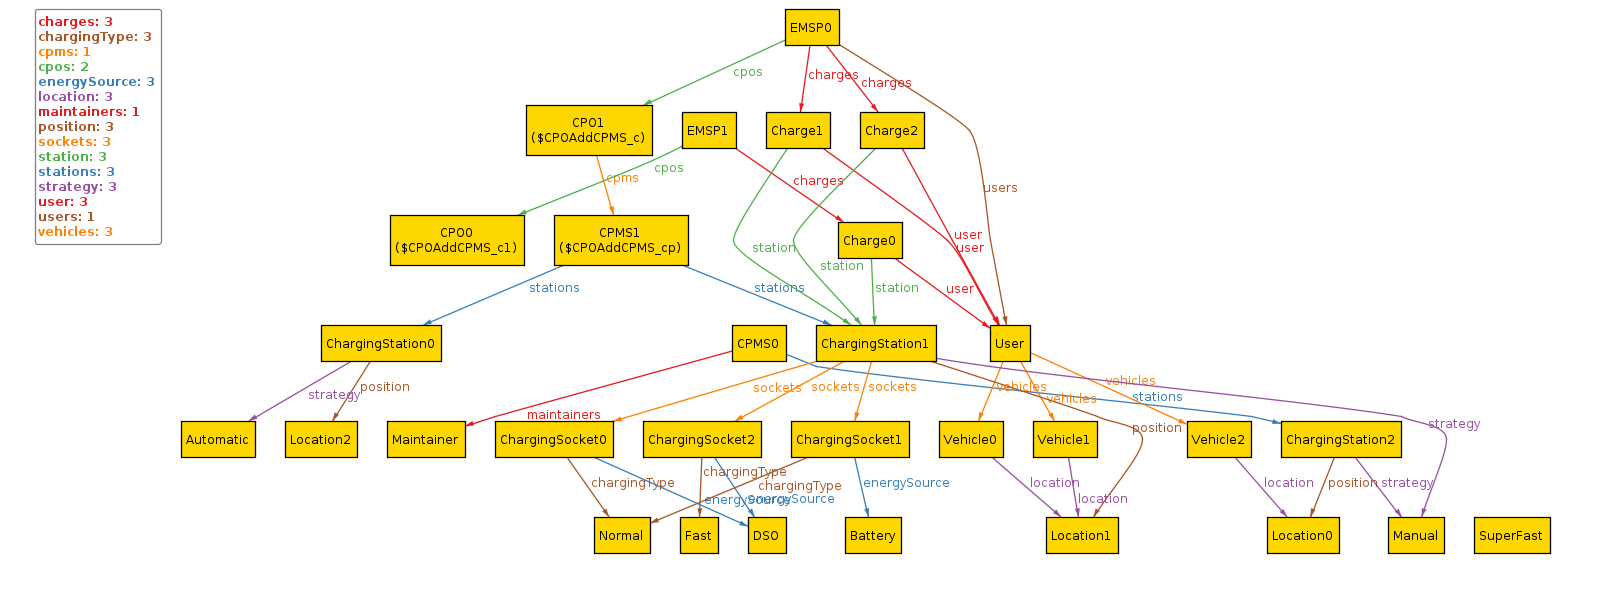
\includegraphics[keepaspectratio, width=16cm]{Alloy/CPOAddCPMS.png}
    \caption{Added CPMS}
\end{figure}

\subsubsection{CPO add mantainer to CPMS}
\begin{verbatim}
    pred CPOAddMantainerToCPMS(c:CPO,cp,cp1:CPMS,m:Maintainer){
        not (cp = cp1)
        cp1 in c.cpms
        cp in c.cpms
        cp.stations=cp1.stations
        cp.maintainers=cp1.maintainers+m
       }
       run CPOAddMantainerToCPMS for 3 but exactly 2 CPMS    
\end{verbatim}
\begin{figure}[H]
    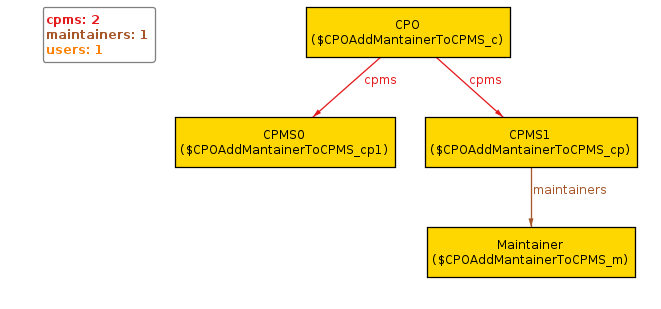
\includegraphics[keepaspectratio, width=16cm]{Alloy/CPoAddMaintainer.png}
    \caption{Added Maintainer}
\end{figure}

\subsubsection{CPO add station to CPMS}
\begin{verbatim}
    pred CPOAddStationToCPMS(c:CPO,cp,cp1:CPMS,s:ChargingStation){
        not (cp = cp1)
        cp1 in c.cpms
        cp in c.cpms
        cp.maintainers = cp1.maintainers
        cp.stations=cp1.stations+s
       }
       run CPOAddStationToCPMS for 3 but exactly 2 CPO    
\end{verbatim}
\begin{figure}[H]
    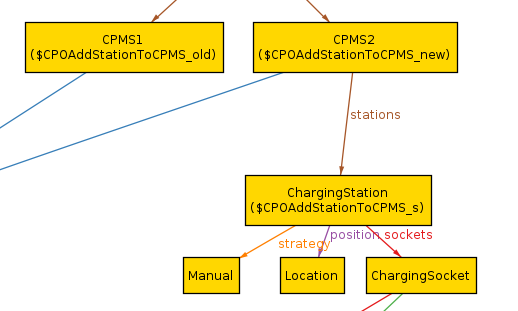
\includegraphics[keepaspectratio, width=16cm]{Alloy/CpoAddStation.png}
    \caption{Added Station}
\end{figure}

\subsubsection{CPO add socket to station}
The following code does not solve, for a limitation of the language,because as a fact a socket can exist only in one station; this is due of the Add patter (s=new station, s1=old station) as for now this pred is never run but supposed as consistent

\begin{verbatim}
    pred CPOAddSocketToStation(c:CPO,cp:CPMS, s,s1:ChargingStation,sk:ChargingSocket){
        not (s = s1)
         cp in c.cpms
         s in cp.stations
         s1 in cp.stations
         s.position=s1.position
         s.strategy=s1.strategy
         s1.sockets=s.sockets+sk
       }
       run CPOAddSocketToStation for 3 but exactly 2 ChargingStation    
\end{verbatim}

\subsection{Assertions}
Here we check the validity of the model trough the Assert notation.
\begin{verbatim}
    assert uniqueLocationForStationCheck{
 	no disjoint s1,s2: ChargingStation | s1.position = s2.position}
check uniqueLocationForStationCheck for 10

assert uniqueCPOForCPMSCheck{
	no disjoint c1,c2: CPO, cp:CPMS | cp in c1.cpms and cp in c2.cpms}
check uniqueCPOForCPMSCheck  for 10

assert uniqueStationForCPMSCheck{
	no disjoint c1,c2: CPMS, s:ChargingStation | s in c1.stations and s in c2.stations}
check uniqueStationForCPMSCheck for 10

assert socketOnlyOneStationCheck{
   all s:ChargingSocket| s in ChargingStation.sockets
	no disjoint c1,c2: ChargingStation, s:ChargingSocket|(s in c1.sockets and s in c2.sockets)}
check socketOnlyOneStationCheck for 10

assert noVehicleWithoutUserCheck{
	all v:Vehicle|  v in User.vehicles}
check noVehicleWithoutUserCheck for 10

assert noStationWithoutCPMSCheck{
	all s:ChargingStation|  s in CPMS.stations}
check noStationWithoutCPMSCheck for 10

assert noUserWithoutEMSP{
	all u:User|  u in EMSP.users}
check noUserWithoutEMSP for 10

assert noChargeWithoutEMSPCheck{
	all c:Charge|  c in EMSP.charges}
check noChargeWithoutEMSPCheck for 10

assert noChargeWithoutUserInTheEMSP{
	all c:Charge| c in EMSP.charges and c.user in EMSP.users}
check noChargeWithoutUserInTheEMSP for 10

assert allChargeAreFromChargingStationInTheSystemCheck{
	all s:Charge.station | s in EMSP.cpos.cpms.stations }
check allChargeAreFromChargingStationInTheSystemCheck for 10

assert maintainersMantainStationOfTheSameCPO{
	all m:Maintainer, c1,c2:CPO|(not c1=c2 and m in c1.cpms.maintainers) implies m not in c2.cpms.maintainers }
check maintainersMantainStationOfTheSameCPO for 10
\end{verbatim}
Which generate the following output.
\begin{figure}[!h]
    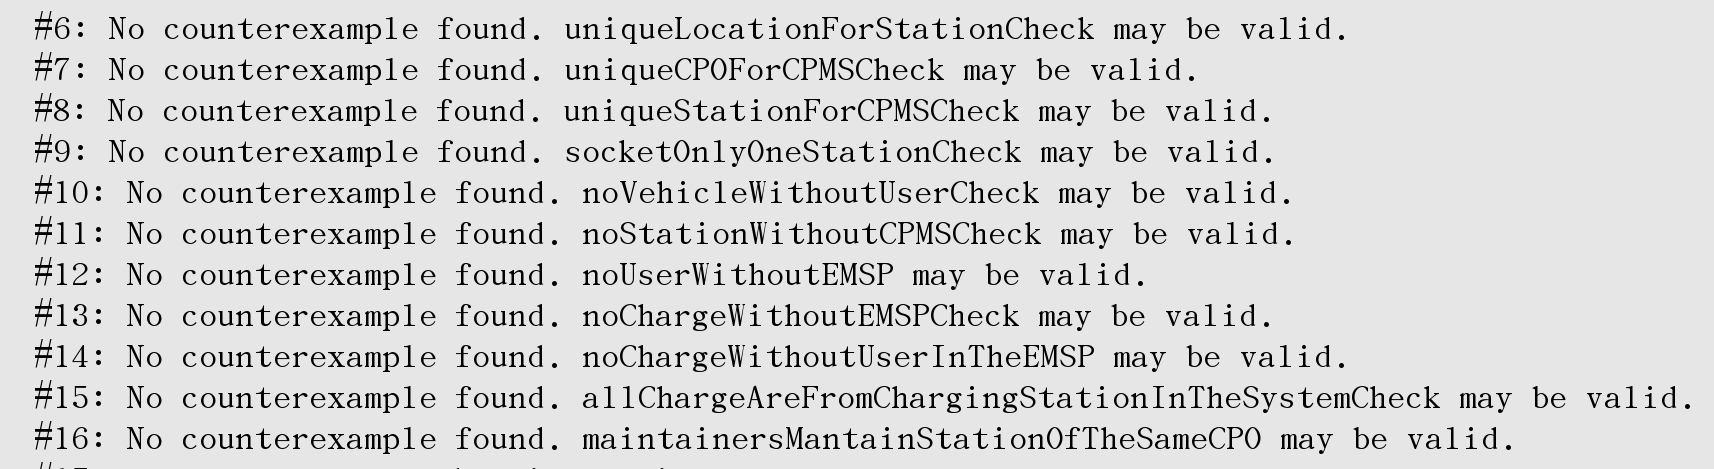
\includegraphics[keepaspectratio, width=16cm]{Alloy/AssertionOutput.png}
    \caption{Assertion output}
\end{figure}
\subsection{Word Generation}
Here is the code of the word generation.
\begin{verbatim}
pred show() {
#EMSP = 1
#CPO>2
#Charge>2
#Vehicle>2
#User>2
}
run show
\end{verbatim}
And the generated word.
\begin{figure}[!h]
    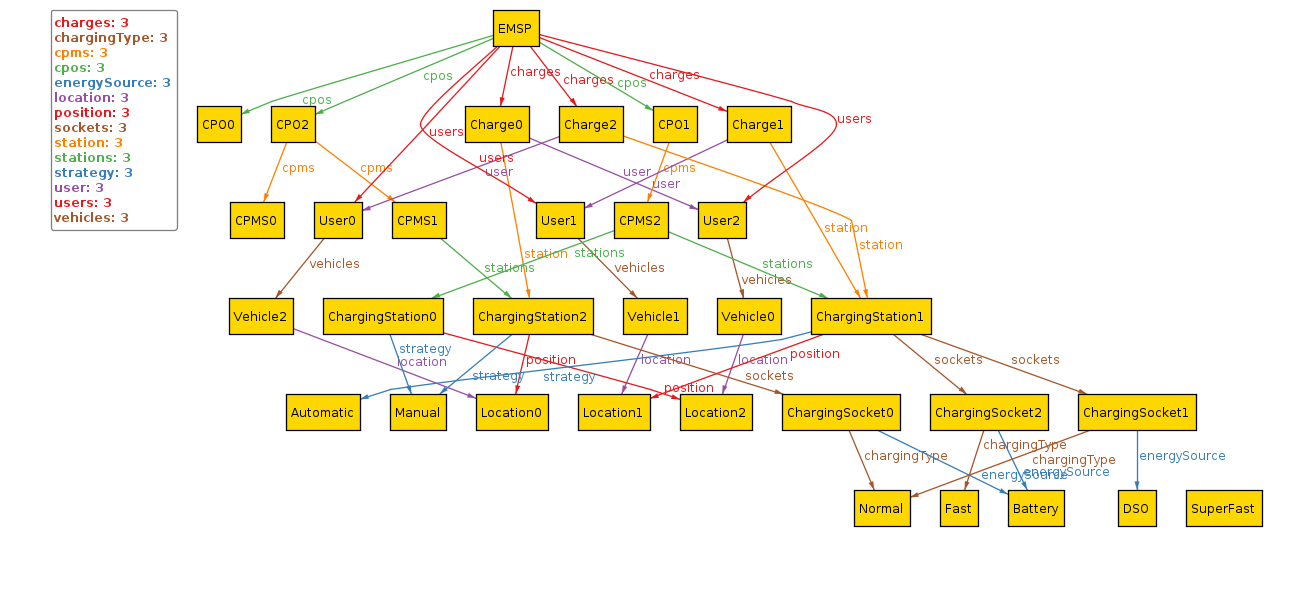
\includegraphics[keepaspectratio, width=16cm]{Alloy/WordResult.png}
    \caption{Generated Word}
\end{figure}
\clearpage